\chapter{Infrastructure as Code (IaC)}
\label{cha:iac}
Infrastructure as Code has become very important with the upcoming of Linux containers and cloud solutions. A developer describes the intended state of the infrastructure via e.g. text files and a tool interprets the description and creates an instance of the infrastructure. With IaC there is no need for manually configuring infrastructures via Graphical User Interfaces (GUI) or Shell anymore. Infrastructures as Code is testable, reproducible and can be vendor independent, because of the abstraction level provided by the description language. 

\section{The Need for IaC}
\label{sec:iac-need}
With IaC, the IT moves from the iron age, to the cloud age [\cite[p. 4]{Morris2017}]. The iron age of the IT, was the time where IT systems were bound to the physical hardware, and a system setup or change was a long term and complex process. In the cloud age of the IT, systems are decoupled from the physical hardware and sometimes even from the underlying operating system. Therefore the setup and change of systems are less complex and can be achieved fast.

The current speed of technological evolution does not support long term processes of infrastructure setup or maintenance anymore. Enterprises with legacy systems see themselves outrun by technological nimble competitors, who can manage infrastructures more efficiently. An Infrastructure setup and the maintenance of the infrastructure in the cloud age has to be simple, trustworthy and fast, otherwise the infrastructures can not cope with the fast changing requirements of the industry.

IaC provides a separation of the infrastructure definition from the underlying operating system and hardware, which in turn allows the automation of the setup and change management of the infrastructure. This can lead to an almost fully automated infrastructure, where changes are applied automatically without the need of a person who has to oversea the process. A common problem which prevents infrastructures to become fully automated is the so called \emph{Automation Fear Spiral} which is shown in figure \ref{fig:automation-fear-spiral}.
\newpage

\begin{figure}[htbp]
	\centering
	%\includesvg{images/automation-fear-spiral}
	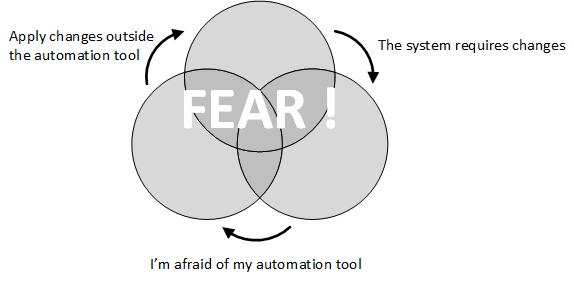
\includegraphics[scale=0.95]{images/automation-fear-spiral.png}
	\caption{Automation Fear Spiral}
	\label{fig:automation-fear-spiral}
\end{figure} 
Because of the missing trust to the automation process and its underlying tooling, changes are applied to the infrastructure manually and outside the defined process. Thus, the infrastructure can become inconsistent, because the changes maybe haven't been added to infrastructure description or change set. If the infrastructure is tried to be reproduced, changes may be missing, because they haven't been added, or are not working because they haven't been tested.

Therefore, teams have to break this spiral to get the automated infrastructure. Additionally, changes which are defined in the infrastructure definitions or separate change sets can be managed by Version Control System (VCS), tested and are therefore consistent and less error prone.

Cloud based solutions make heavy usage of IaC, because the cloud providers can not allow the developers to tamper with the underlying system. With the definition language, the cloud providers provide an abstraction of the underlying system and an easy way to define the infrastructure for the specific cloud solution. The developers only have to describe the infrastructure and its changes, the cloud providers are responsible to create an instance of the infrastructure and to apply changes to it. Therefore, the developers can spend more time on the definition of the infrastructure their applications need.

\section{Principles of IaC}
\label{sec:iac-principles}
